\documentclass[aspectratio=169, hyperref={pdfpagelabels=false}]{beamer}
%\usepackage{helvet}
%\renewcommand{\familydefault}{\rmdefault}
\usepackage{mathpazo}
\usefonttheme{professionalfonts}
\usefonttheme{serif}
\usepackage[english]{babel}
\usepackage{pgfplots}
\usepackage{pgf}
\usepackage{pgfpages}
\pgfplotsset{compat=newest}
\usepackage{booktabs}
\usepackage[T1]{fontenc}
\usepackage[utf8]{inputenc}
\usepackage{lipsum}
\usepackage{tcolorbox}
\usepackage{xcolor}
\usepackage{listings}
\usepackage{microtype}
\usepackage{float}
\usepackage{siunitx}
\usepackage{multicol}
\usepackage{hyperref}
\usepackage{dsfont}
\usepackage{caption}
\usepackage{subcaption}
\usepackage{dashbox}
\usepackage{csquotes}
\usepackage[absolute, overlay]{textpos}

\setlength{\TPHorizModule}{\textwidth}
\setlength{\TPVertModule}{\textwidth}

% DTU colours for diagrams
% You might want to make the front/back page background colour the first colour in the plot cycle list.
\pgfplotscreateplotcyclelist{DTU}{%
dtured,         fill=dtured,        \\%
blue,           fill=blue,          \\%
brightgreen,    fill=brightgreen    \\%
navyblue,       fill=navyblue       \\%
yellow,         fill=yellow         \\%
orange,         fill=orange         \\%
grey,           fill=grey           \\%
red,            fill=red            \\%
green,          fill=green          \\%
purple,         fill=purple         \\%
}

% Table of contents (TOC) and numbering of headings
\setcounter{tocdepth}{1}    % Depth of table of content: sub sections will not be included in table of contents
\setcounter{secnumdepth}{2} % Depth of section numbering: sub sub sections are not numbered



\newcommand{\setcolor}[1]{\def\chosencolor{#1}}
\newcommand{\setdepartment}[1]{\def\department{#1}}

\DeclareMathOperator*{\argmax}{argmax}
\DeclareMathOperator*{\argmin}{argmin}
\DeclareMathOperator{\E}{\mathbb{E}}

\newcommand{\indep}{\perp \!\!\! \perp}

\usetheme{DTU}
\setbeamersize{text margin left=22mm}
\def\insertframetitle{}

\newcommand{\inserttitlepage}{
    \begin{frame}[plain, noframenumbering]{}

        \begin{center}
        \hspace{-3.6em}
            
\includegraphics[width = 0.25\paperwidth]{logos/\targetcolourmodel/white.pdf}
        \end{center}
        
    \end{frame}

    \begin{frame}[plain]{}
        \color{white}\maketitle
    \end{frame}

    \setbeamercolor{background canvas}{bg = white}
}


%\AtBeginSection[]{
%  \begin{frame}[plain, noframenumbering]{}
%        %\usebeamercolor[fg]{title}
%        
%        % title
%               {\Large\insertsubtitle\par}\vspace{2mm}
%               {\usebeamerfont{title}\textbf{\insertsectionhead\par}\par}\vspace{5mm}
%               {\Large\insertauthor\par}\vspace{5mm}
%  \end{frame}
%    }





%% Algorithm
\newcounter{nalg} % defines algorithm counter
\renewcommand{\thenalg}{\arabic{nalg}} %defines appearance of the algorithm counter
\DeclareCaptionLabelFormat{algocaption}{Algorithm \thenalg} % defines a new caption label as Algorithm x.y
\definecolor{cadet}{rgb}{0.33, 0.41, 0.47}
\lstnewenvironment{algorithm}[1][] %defines the algorithm listing environment
{   
    \refstepcounter{nalg} %increments algorithm number
    \captionsetup{labelformat=algocaption,labelsep=colon} %defines the caption setup for: it ises label format as the declared caption label above and makes label and caption text to be separated by a ':'
    \lstset{ %this is the stype
        mathescape=true,
        frame=tB,
        numbers=left, 
        numberstyle=\tiny,
        basicstyle=\scriptsize\ttfamily, 
        keywordstyle=\color{black}\bfseries,
        keywords={,optional, input, output, return, datatype, function, if, else, for, foreach, begin, end, } %add the keywords you want, or load a language as Rubens explains in his comment above.
        numbers=left,
        xleftmargin=.04\textwidth,
        morecomment=[l][\color{cadet}]{//},
        #1 % this is to add specific settings to an usage of this environment (for instnce, the caption and referable label)
    }
}
{}


\newcommand{\highlight}[1]{%
  \colorbox{blue!20}{$\displaystyle#1$}}


\newcommand{\mybox}[2]{\begin{textblock}{0.4}(#1)\dbox{
    \begin{minipage}{\dimexpr\textwidth-2\fboxsep-2\fboxrule\relax}
    \scriptsize
    #2
    \end{minipage}}\end{textblock}}
\usepackage[
  style=authoryear-comp,
  maxnames=2,
  backend=biber,
  safeinputenc,
  isbn=false,
  doi=false,
  maxcitenames=2,
  date=year]{biblatex}
 
\addbibresource{Defence bibliography.bib}


% To give a presentation with the Skim reader (http://skim-app.sourceforge.net) on OSX so
% that you see the notes on your laptop and the slides on the projector, do the following:
% 
% 1. Generate just the presentation (hide notes) and save to slides.pdf
% 2. Generate onlt the notes (show only nodes) and save to notes.pdf
% 3. With Skim open both slides.pdf and notes.pdf
% 4. Click on slides.pdf to bring it to front.
% 5. In Skim, under "View -> Presentation Option -> Synhcronized Noted Document"
%    select notes.pdf.
% 6. Now as you move around in slides.pdf the notes.pdf file will follow you.
% 7. Arrange windows so that notes.pdf is in full screen mode on your laptop
%    and slides.pdf is in presentation mode on the projector.

%\setbeameroption{show notes}
\setbeameroption{hide notes} % Only slides
%\setbeameroption{show only notes} % Only notes
%\setbeameroption{show notes on second screen=right} % Both

\subtitle{Ph.D. thesis defence}
\title{Programmatic Agents and Causal State Abstractions}
\author{Rasmus Larsen}

\setdepartment{DTU Compute}
\setcolor{dtured}


\begin{document}
\inserttitlepage

\note{Today I will be giving an overview of my research in structured abstractions of states and policies in reinforcement learning.}


%\begin{frame}{Overview}
%\tableofcontents
%\end{frame}

\section{Motivation}
\begin{frame}{Motivation}
\begin{itemize}
    \item Everyone can probably agree: The AI of today is narrow.
    \item Issues: Generalization, trust, 
    
    \item What motivated my work was the identification of three crucial factors for increased AI capability: Compositionality, communicability, and state abstraction.
\end{itemize}
\end{frame}

\note[itemize]{
    \item AI needs to be able to deal with situations outside of those with cheap, plentiful data. Generalize to novel situations that are completely unseen.
    \item Can we trust narrow AI? When?
}

\begin{frame}{Theme: Robot in a kitchen}
    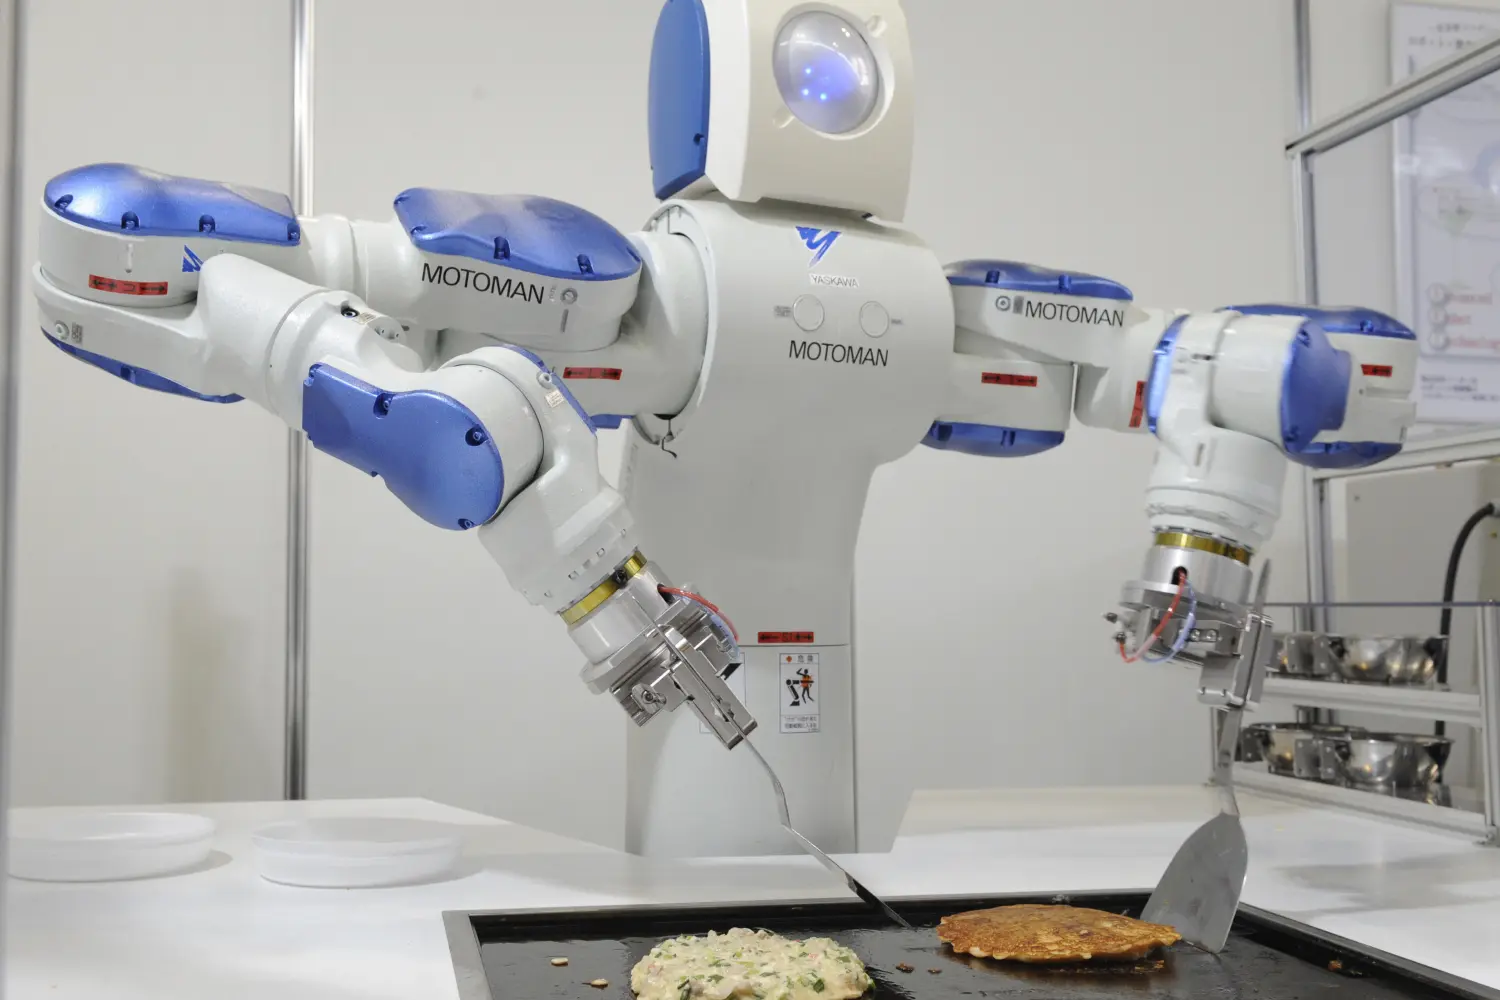
\includegraphics[width=.7\textwidth]{images/robot-cooking.png}
\end{frame}

\note[itemize]{
    \item I'm going to be using references to kitchen scenarios several times
    \item So I wanted to give you an image you could think of whenever I do
    \item These scenarios are relatable yet quite difficult.
    \item Directly motivates the 3 features.
}

\begin{frame}{Composition}
\begin{itemize}
    \item Recipes.
    \item There is never enough data to cover every case in the real world.
    \item 
\end{itemize}
\end{frame}

\note[itemize]{
    \item 
}

\begin{frame}{Communication}
\begin{itemize}
    \item 
    \item 
\end{itemize}
\end{frame}

\begin{frame}{State abstraction}
    \begin{itemize}
        \item 
        \item 
    \end{itemize}
    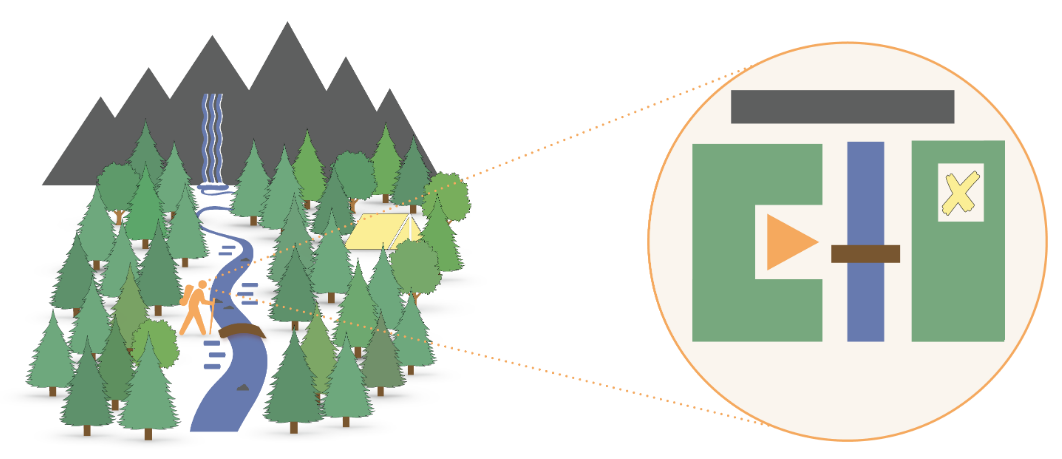
\includegraphics[width=0.58\textwidth]{images/valueofabstraction.png}
    \mybox{0.7, 0.35}{\fullcite{hoValueAbstraction2019}}
\end{frame}

\begin{frame}{Reinforcement Learning setting}
    
\end{frame}

\begin{frame}{Nethack challenge}
\begin{itemize}
    \item Symbolic manipulation agent beat DL by far. 
\end{itemize}
\end{frame}

\begin{frame}{Overview}
% not TOC
    
\end{frame}

\note[itemize]{
    \item test1
    \item test2
}

\part{Programmatic policies}
\frame[noframenumbering]{\centering\partpage\strut}
\section{Programmatic policies}
\begin{frame}{Programmatic policies}
    \begin{itemize}
        \item \textbf{Differentiable control policies}
        \begin{itemize}
            \item Mainly used for optimization reasons.
            \item In general lack: explainability, compositionality, generalization, inductive bias.
        \end{itemize}
        \item \textbf{Programmatic policies}
        \begin{itemize}
            \item Compositional and inherently explainable.
            \item Domain specific languages provide inductive bias and generalization.
            \item Optimization is very difficult.
        \end{itemize}
    \end{itemize}
    \mybox{0.7, 0.43}{\fullcite{larsenProgrammaticPolicyExtraction2022}}
\end{frame}

\note[itemize]{
    \item I covered the overall motivation for my work, but here's some specific points relating that to this particular work.  
}

\begin{frame}{Approach: Extracting programs from black-box policies}
\begin{itemize}
    \item How to integrate programmatic policy representations with reinforcement learning?
    \item Bellman equation tells us nothing about how to improve a programmatic policy.
    \bigskip
    \item \textbf{Key idea:} Extracting programs from existing policies.
\end{itemize}
\end{frame}

\note[itemize]{
    \item So what can we do? We don't know how to learn directly in program space.
    \item In principle, each program has to be "experimented with" in the environment.
    \item At least, that's the case unless we have a model of how \emph{syntactic} changes result in changes to the agents state distribution and thus obtained reward.
    \item One approach is to bootstrap on existing RL algorithms
    \item Given a trained policy, we can try to extract a program that imitates it.
    \item This has some advantages, such as being compatible with future improvements to RL algorithms.
}

\begin{frame}{Background: Behavioral cloning}
    \begin{itemize}
        \item The simplest way to learn from action demonstrations.
        \item With access to an \emph{expert} $f(x)$, obtain supervised dataset $\{(x_i, f(x_i))\}$.
        \item In RL setting with expert policy $\pi(s)$: Obtain trajectories $\{(s_i, \pi(s_i)\} \sim p_\pi(s)$.
        \item Key issue: Expert only visits \enquote{good} states.
    \end{itemize}
    
    \mybox{0.7, 0.45}{\fullcite{bainFrameworkBehaviouralCloning1999}}
\end{frame}

\note[itemize]{
    \item I'm going to start with some background on methods, building up to my work.
    \item Okay, so how would we go about integrating RL and programs.
    \item The Bellman equation says nothing about improving programs.
    \item It does tell us how to evaluate a given program, though.
    \item The approach here is going to be one where we *somehow* obtain a black-box policy - for example, these days, by using existing Deep RL methods to learn a NN encoding the policy in its weights.
    \item Then, the goal is to extract information from this policy and into a program. That is, we want to obtain a good clone of the black-box policy as a structured program.
    \item There is a really well-known, important problem with BC.
    \item As in any supervised learning problem, the dataset must be representative of the problem.
    \item If we don't have supervision in some part of the state space, the data tells the student nothing about how to act.
    \item Student performance thus degrades as soon as it veers off the expert path.
}

\begin{frame}{Background: Dataset Aggregation}
    \begin{itemize}
        \item Perhaps the first example of \emph{interactive} imitation.
        \item Conceptually simple: At the first iteration, it uses the expert’s policy to gather a dataset of trajectories $\mathcal{D}$ and train a student $\hat\pi_2$ that best mimics the expert on those trajectories. 
        \item Then at iteration $n$, it uses $\hat\pi_n$ to collect more trajectories and adds those trajectories to the dataset $\mathcal{D}$.
    \end{itemize}
    
    \mybox{0.7, 0.42}{\fullcite{rossReductionImitationLearning2011}}
\end{frame}

\note[itemize]{
    \item As I mentioned, this is a well-known issue.
    \item A solution is to do what I would call interactive imitation. Dataset Aggregation or DAgger is an early example of interactive imitation.
    \item It achieves good performance guarantees under the induced state distribution of the final student policy.
    \item It works as follows: <follow screen>
    \item Of course, states are generated by the student in subsequent iterations, BUT actions are still labelled by the expert for the dataset!
}

\begin{frame}[fragile]{Background: Imitation-Projected RL}
\begin{algorithm}[caption={Imitation-Projected Programmatic Reinforcement Learning}]
 input: initial (neural) policy $\pi_0$
 output: joint policy $h_J$, program $p_J$
 $p_0 \leftarrow \textsc{Project}(\pi_0)$
 for $j = 1, \dots, J$
   $h_j \leftarrow \textsc{Update}(p_{j-1}) \quad$ // standard RL algorithm
   $p_j \leftarrow \textsc{Project}(h_j)$
 end
\end{algorithm}

\begin{itemize}
    \item A generic framework for combining RL and structured policies through imitation learning.
\end{itemize}

\mybox{0.7, 0.46}{\fullcite{vermaProgrammaticallyInterpretableReinforcement2018}}
\end{frame}

\note[itemize]{
    \item With that in mind, let's move on to considering structured policies.
    \item Imitation-Projected RL is the starting point for my work with programmatic policies.
    \item It is indeed a framework for the problem that I started this section discussing: imitating a policy with a structured policy. 
    \item It consists of iterating two steps, which we call update and project.
    \item Update takes the current policy and improves it, that is: its a standard RL algorithm.
    \item Project takes this updated policy and projects it into program space.
    \item As the name of the framework suggests, this projection is performed by imitation.
}

\begin{frame}[fragile]{Imitation-Projected RL II}
The imitation-projection operator $\textsc{Project}$ is implemented using an interactive imitation learning algorithm, such as DAgger \citep{ross2011reduction}.

\begin{algorithm}[caption={$\textsc{Project}$: imitation learning}]
 input: structured policy class $\mathcal{P}$
 input: oracle policy $h$
 output: structured imitation policy $p_K$
 $\tau_0 \leftarrow $ $N$ on-policy trajectories using $h$
 create supervised dataset $\Gamma_0 = \left\{\left(s, h(s)\right) |\, s \in \tau_0 \right\}$
 $p_0 \leftarrow \textsc{Derive}(\mathcal{P}, \Gamma_0)$
 for $k = 1, \dots, K$
   $\tau_k \leftarrow $ $M$ on-policy trajectories using $p_{k-1}$
   create supervised dataset $\Gamma' = \left\{\left(s, h(s)\right) |\, s \in \tau_k \right\}$
   aggregate datasets: $\Gamma_k = \Gamma_{k-1} \cup \Gamma' \quad$
   $p_k \leftarrow \textsc{Derive}(\mathcal{P}, \Gamma_k)$
 end
\end{algorithm}

In the framework, $\textsc{Derive}$ is an unspecified function that maps a dataset $\Gamma$ to a member of the set of policies $\mathcal{P}$ that imitates the dataset well.


\end{frame}




\begin{frame}[fragile]{Imitation-Projection with program synthesis}
\textsc{Derive} was implemented as a search over parameterized PID controllers or simple decision trees.

\begin{itemize}
    \item These spaces are inflexible and small enough to enumerate.
    \item Extension 1: More general, flexible space of programmatic policies.
    \item Extension 2: $\textsc{Derive}$ should improve on previous solutions.
\end{itemize}

\begin{algorithm}[caption={$\textsc{Project}$: imitation learning by improvement}]
 $\dots$
 for $k = 1, \dots, K$
   $\tau_k \leftarrow $ $M$ on-policy trajectories with $p_{k-1}$
   create supervised dataset $\Gamma' = \left\{\left(s, h(s)\right) |\, s \in \tau_k \right\}$
   aggregate datasets: $\Gamma_k = \Gamma_{k-1} \cup \Gamma' \quad$
   $p_k \leftarrow \textsc{Derive}(\Gamma_k, \highlight{\{p_0,\,\dots,\,p_{k-1}\}})$
 end
\end{algorithm}
\end{frame}

\note[itemize]{
    \item 
}

\begin{frame}{Instantiation: \textsc{Derive} by typed neighborhood search I}
    Many potential instantiations -- we experimented with a relatively straightforward one.
    \begin{itemize}
        \item \textbf{Main concept:} Improve on the latest discovered solution by greedily searching through its neighborhood.
        \item \textbf{Program space:} Domain Specific Language defined in the lambda calculus with HM type system.
        \item \textbf{Search method:} Enumeration of a depth-limited type-directed neighborhood.
        \item Importantly, the neighborhood search is repeated $K$ times per projection, as shown in the definition of $\textsc{Project}$.
        \item Does this iterative framework allow for better interactive imitation learning using program representations?
        %\item Given a DSL $\mathcal{D}$ of typed functions and constants, we define the result of the operator $\textsc{edit}(P, l, P')$ as the program obtained by replacing the subprogram at location $l$ in $P \in \mathcal{D}$ by $P' \in \mathcal{D}$.
        %\item The neighborhood $N_n^d(\mathcal{D}, P)$ of program $P$ is defined as all well-typed programs generated by applying $\textsc{edit}$ at all locations $l$ using all valid substitutions $P'$, where $size(P') < d$ and with up to $n$ simultaneously applied edits.
        %\item During edit generation, the expression at $l$ in $P$ is temporarily added to the DSL.
    \end{itemize}
\end{frame}

\begin{frame}[fragile]{Instantiation: \textsc{Derive} by typed neighborhood search II}
Example of a DSL:
\begin{itemize}
    \item Constants: $(\texttt{Bool: \{true, false\}, Int: \{0, 1, 2\}})$
    \item Functions: $\begin{aligned}
        (&\texttt{add :: Int -> Int -> Int}, \\
         &\texttt{if :: $\forall$a. Bool -> a -> a -> a})
    \end{aligned}$
\end{itemize}

The neighborhood of program $p$ is here defined based on all well-typed substitutions $p'$ into $p$ of size less than $d$ at all locations in the AST of $p$. Example of a neighborhood:
\begin{itemize}
    \item $p: \texttt{add 1 1}$.
    \item Neighbors: $\texttt{? :: Int $\cup$ add (? :: Int) 1 $\cup$ add 1 (? :: Int)}$.
    \item Example neighbor: $\texttt{if True (add 1 2) 0}$.
    \item Example neighbor: $\texttt{add 1 (add 1 1)}$.
\end{itemize}
\end{frame}

\begin{frame}[fragile]{Instantiation: \textsc{Derive} by typed neighborhood search III}
    \begin{algorithm}[caption={Greedy search in the depth-limited typed neighborhood}]
     input: domain specific language $\mathcal{D}$
     input: imitation dataset $\Gamma$
     input: initial program $P$
     output: best program in typed neighborhood $p^*$
     function $N_n^d(\mathcal{D},\, P,\, l) \quad$ // generates the neighborhood for location $l$ in $P$
       return $\varnothing$ if d = 0
       $T \leftarrow $ type of expression at $l$ in $P$
       $C \leftarrow $ everything from $\mathcal{D}$ whose type $t$ can unify with $T$
       $P' \leftarrow $ all substitutions of expressions from $C$ into $P$
       return complete programs in $P' \cup N_n^{d-1}$ of all partial programs 
     end
     $N_n^d \leftarrow \bigcup_{l \in L_n(P)}N_n^d(\mathcal{D},\, P,\, l)$
     $p^* \leftarrow \argmax_{p \in N_n^d}\textsc{eval}(p, \Gamma)$ 
    \end{algorithm}
\end{frame}

\begin{frame}{Results}
    \begin{figure}
      %\centering
      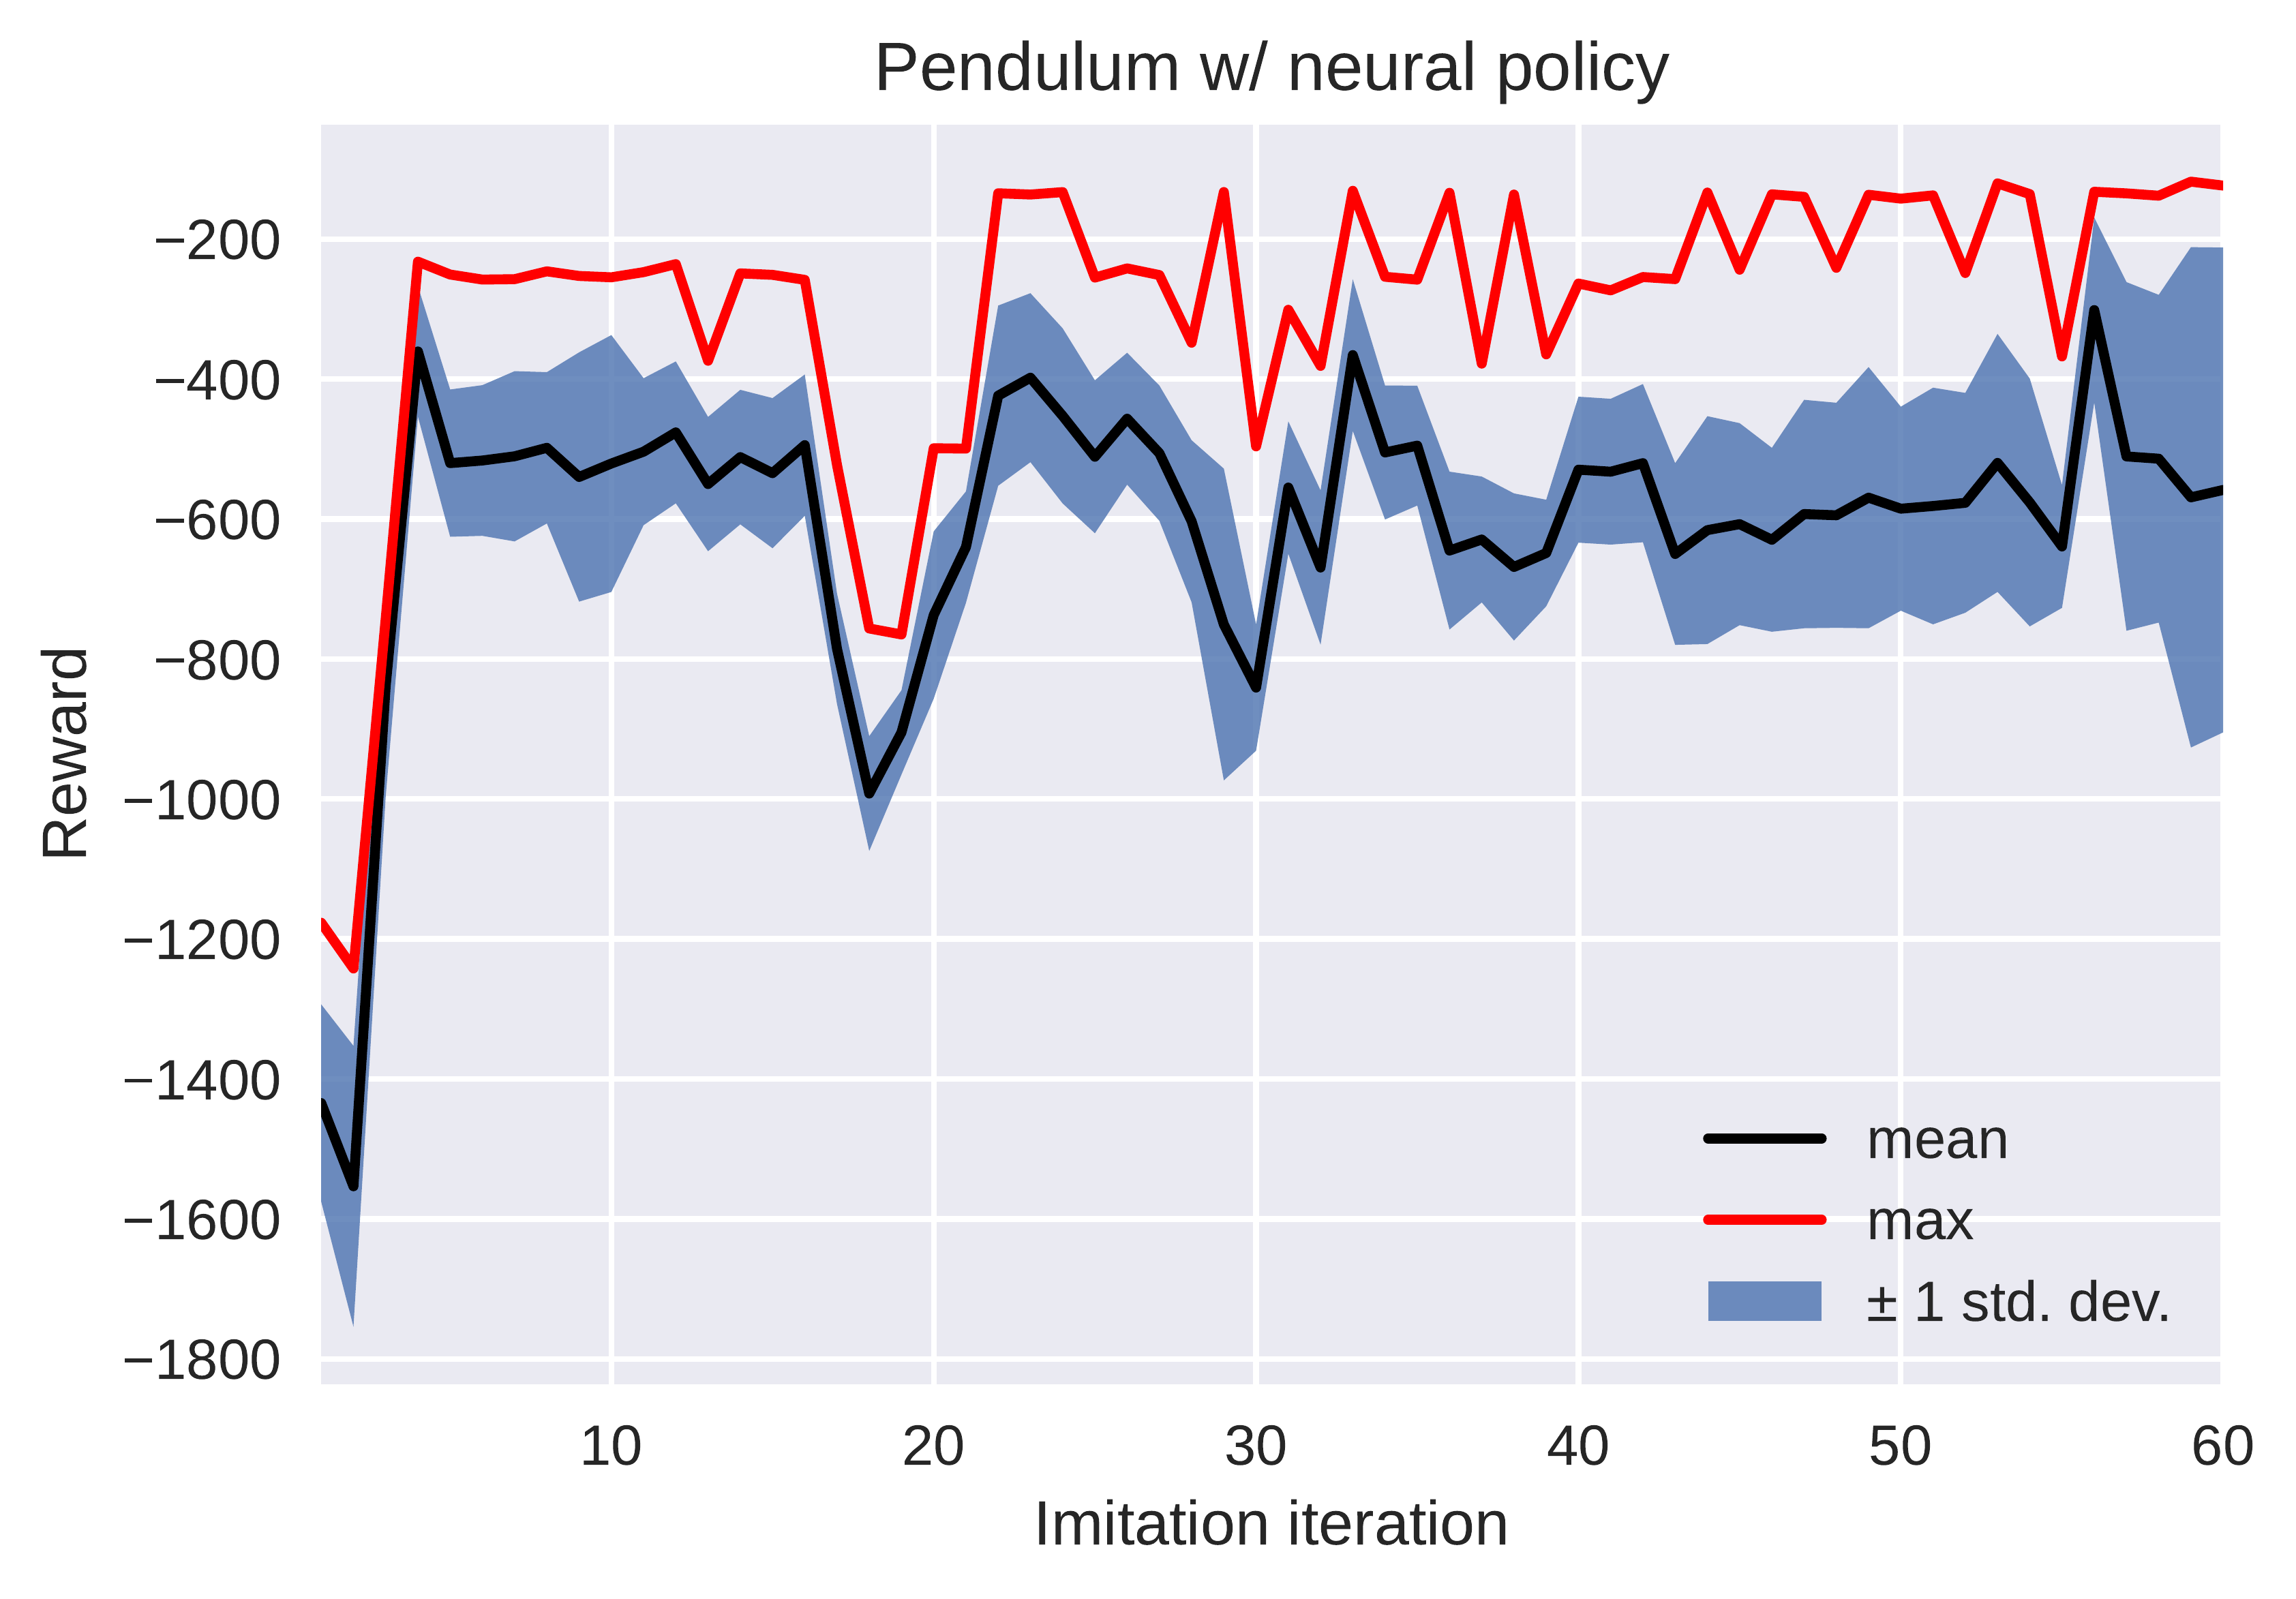
\includegraphics[width=0.37\textwidth]{images/performance.png}
      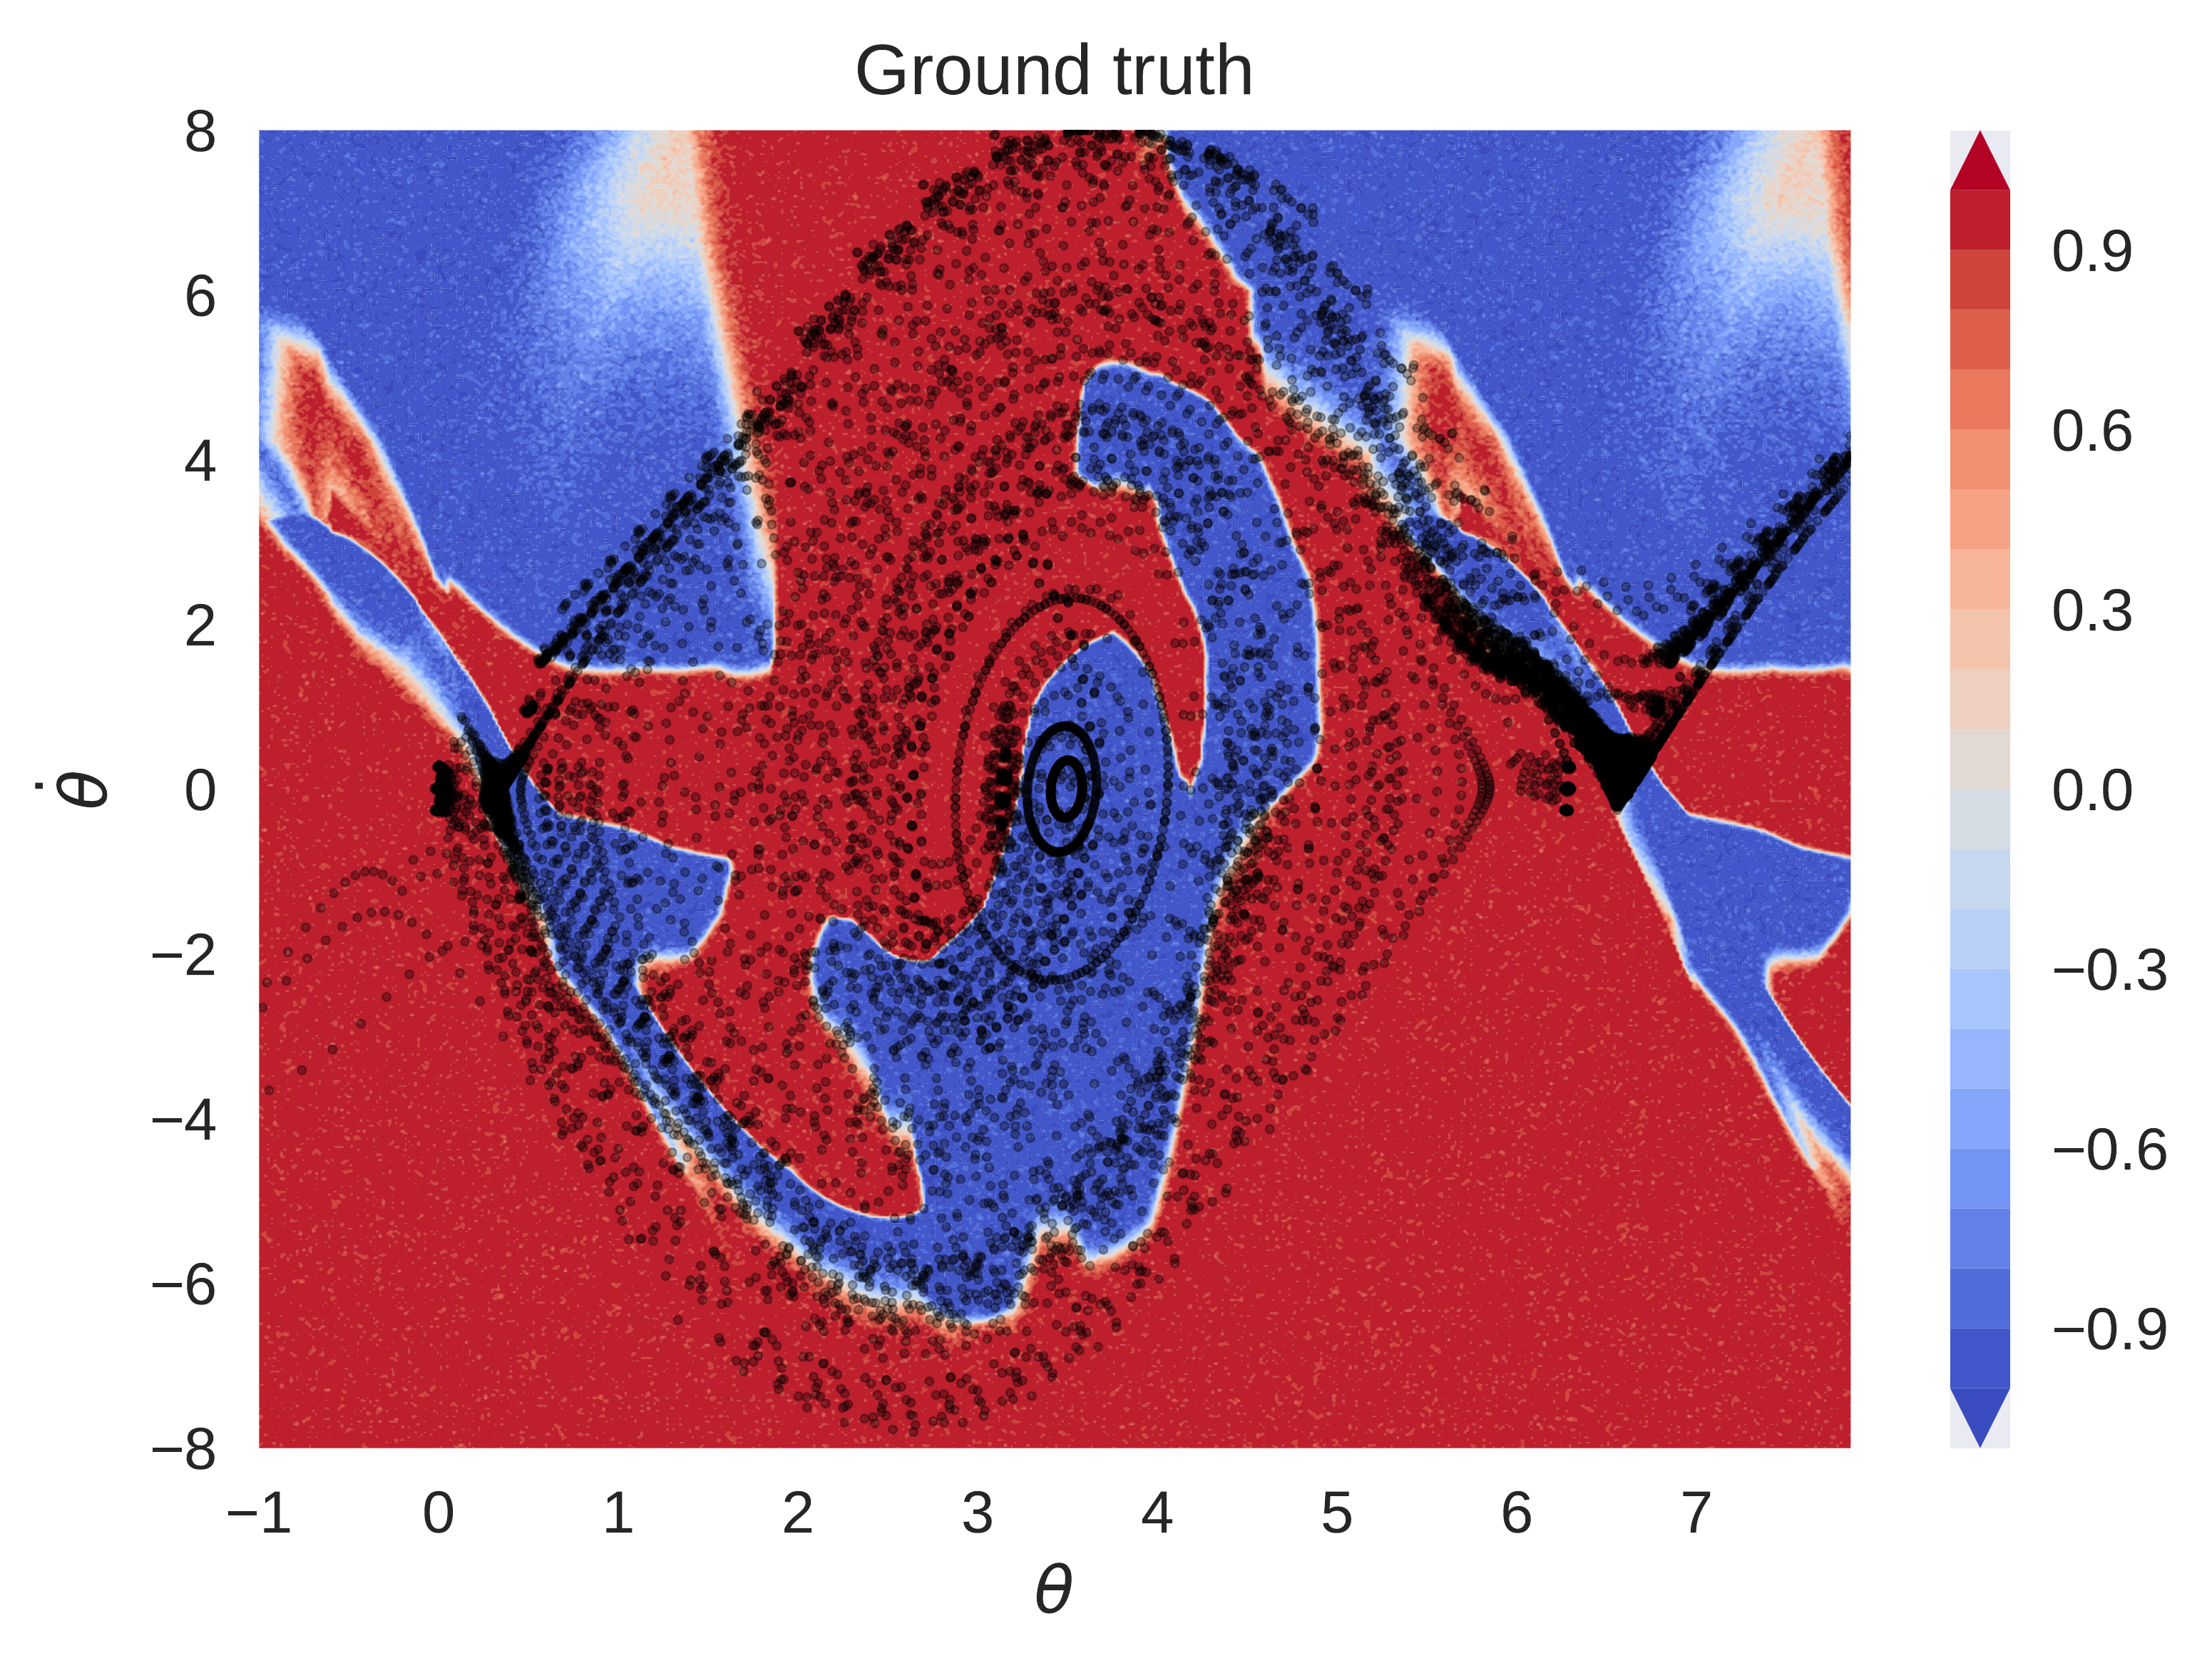
\includegraphics[width=0.37\textwidth]{images/groundtruth.png}
      
      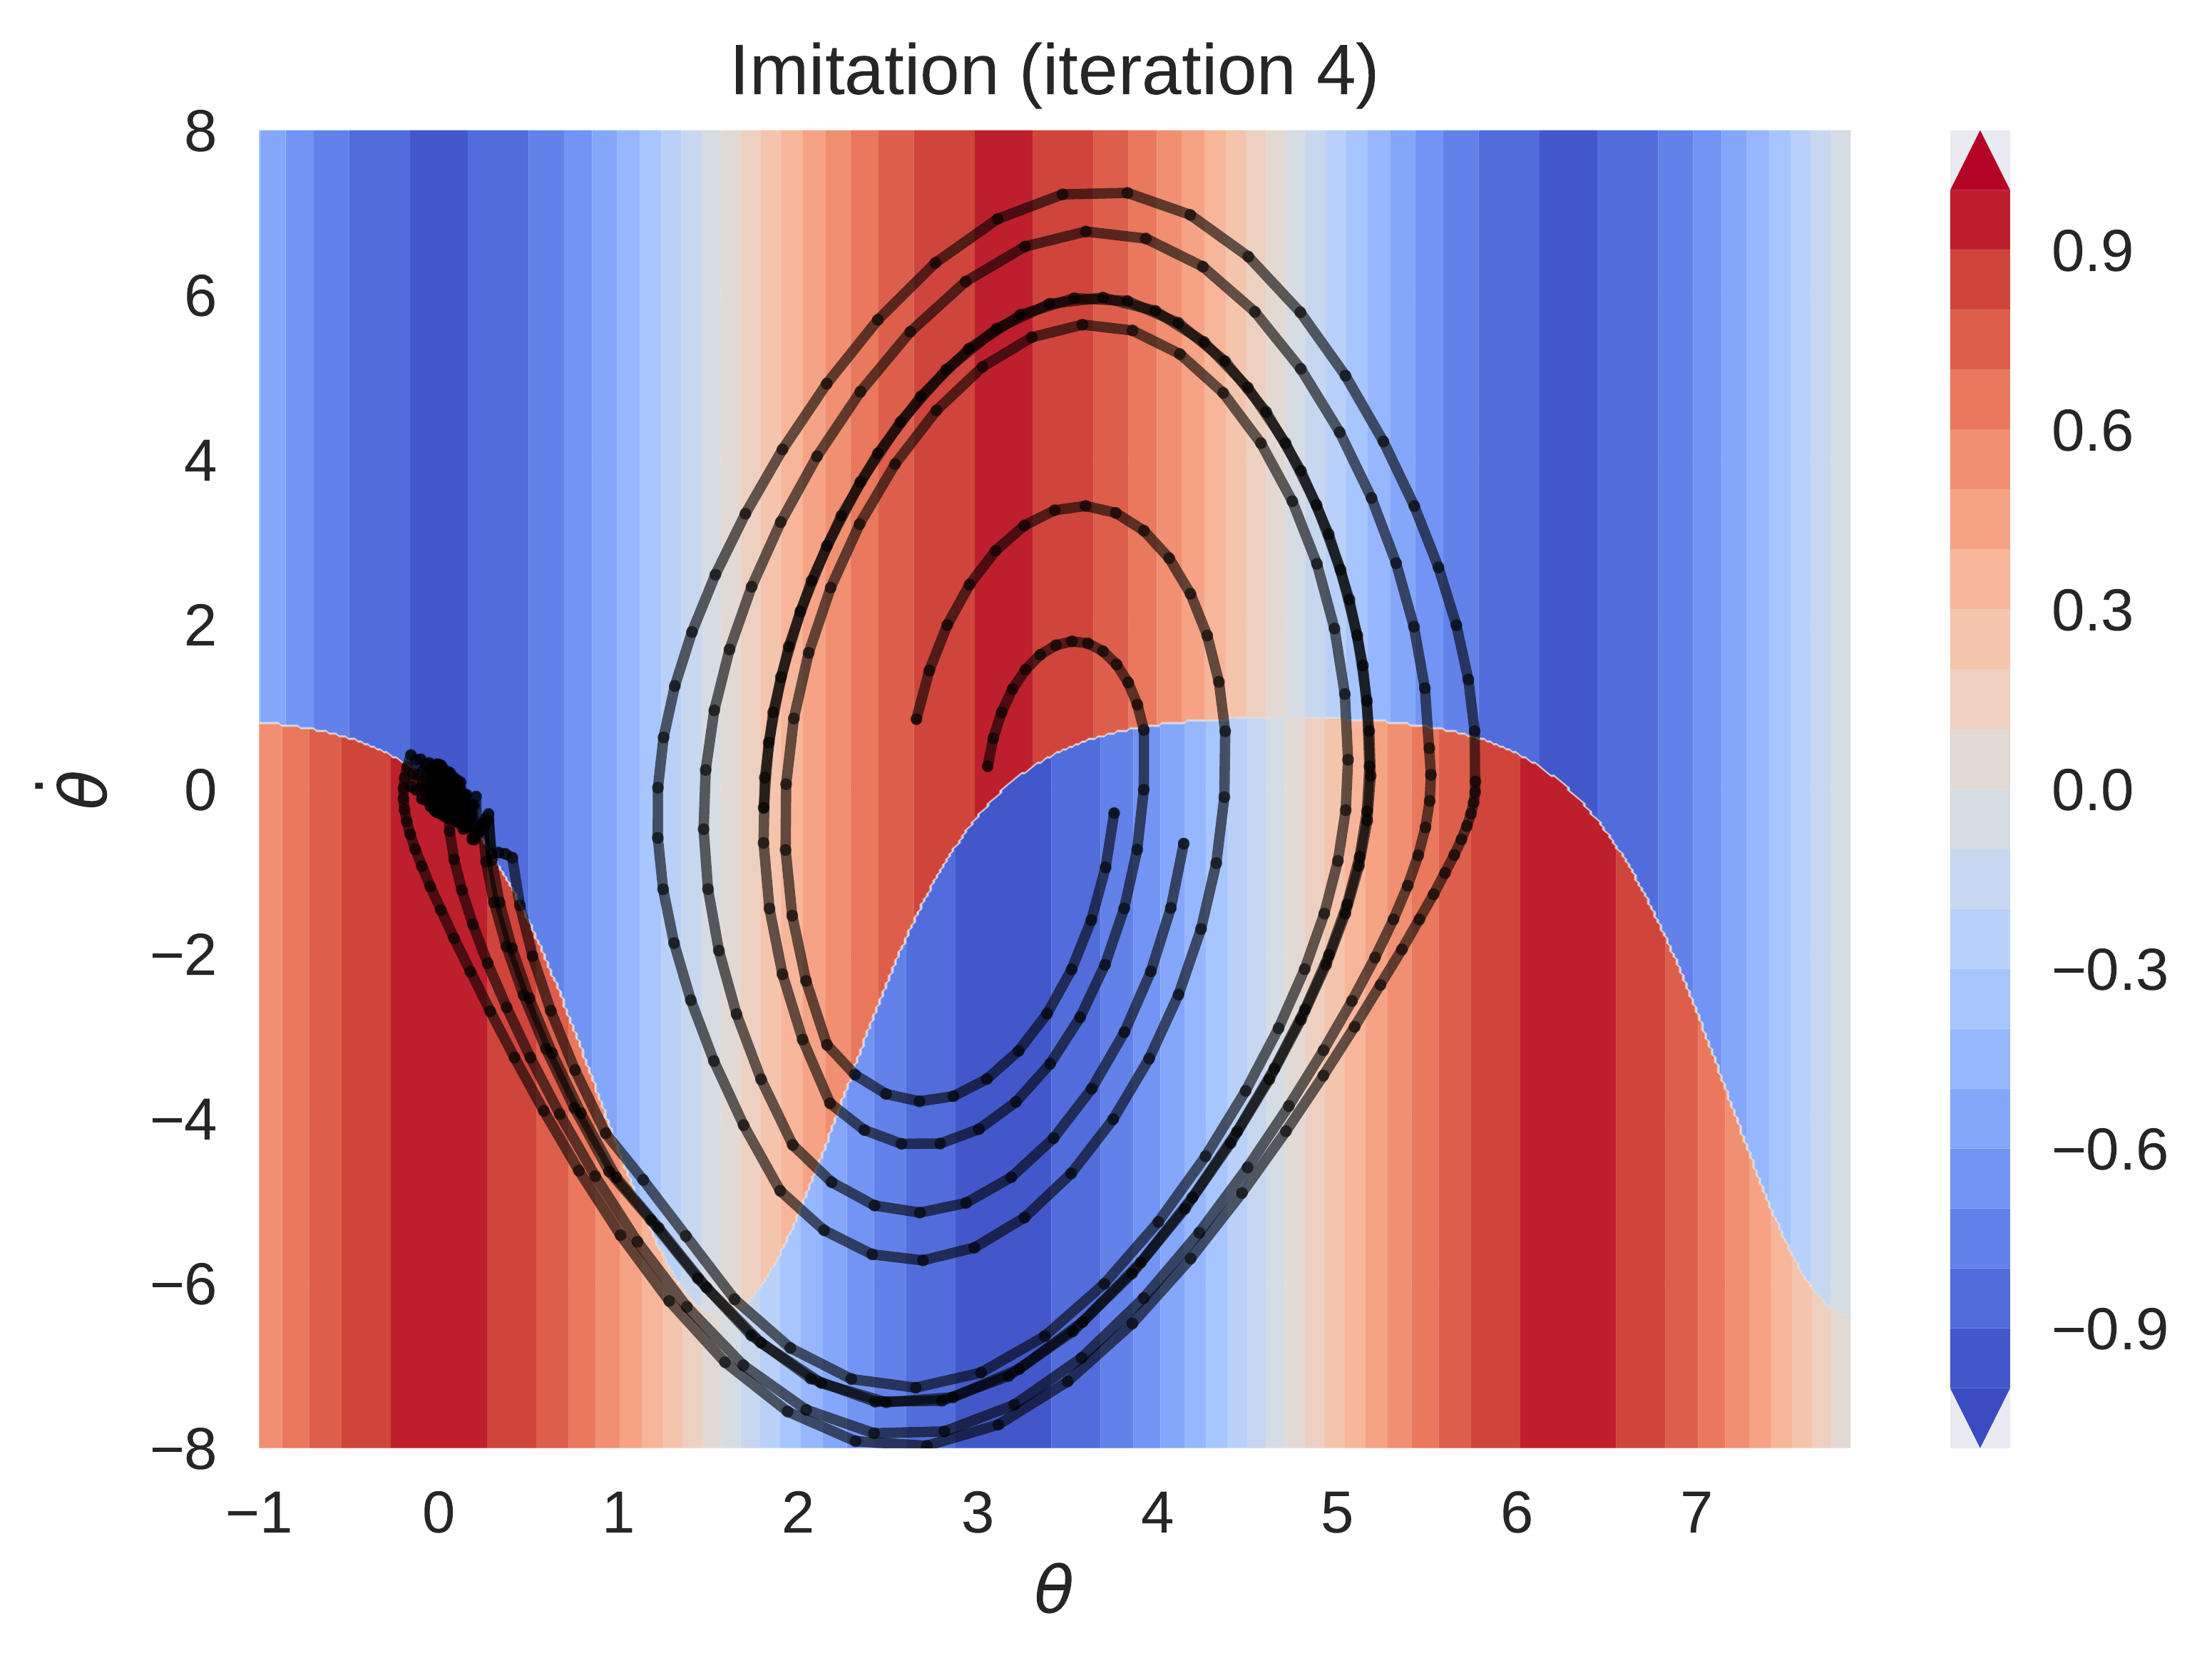
\includegraphics[width=0.37\textwidth]{images/imitation4.png}
      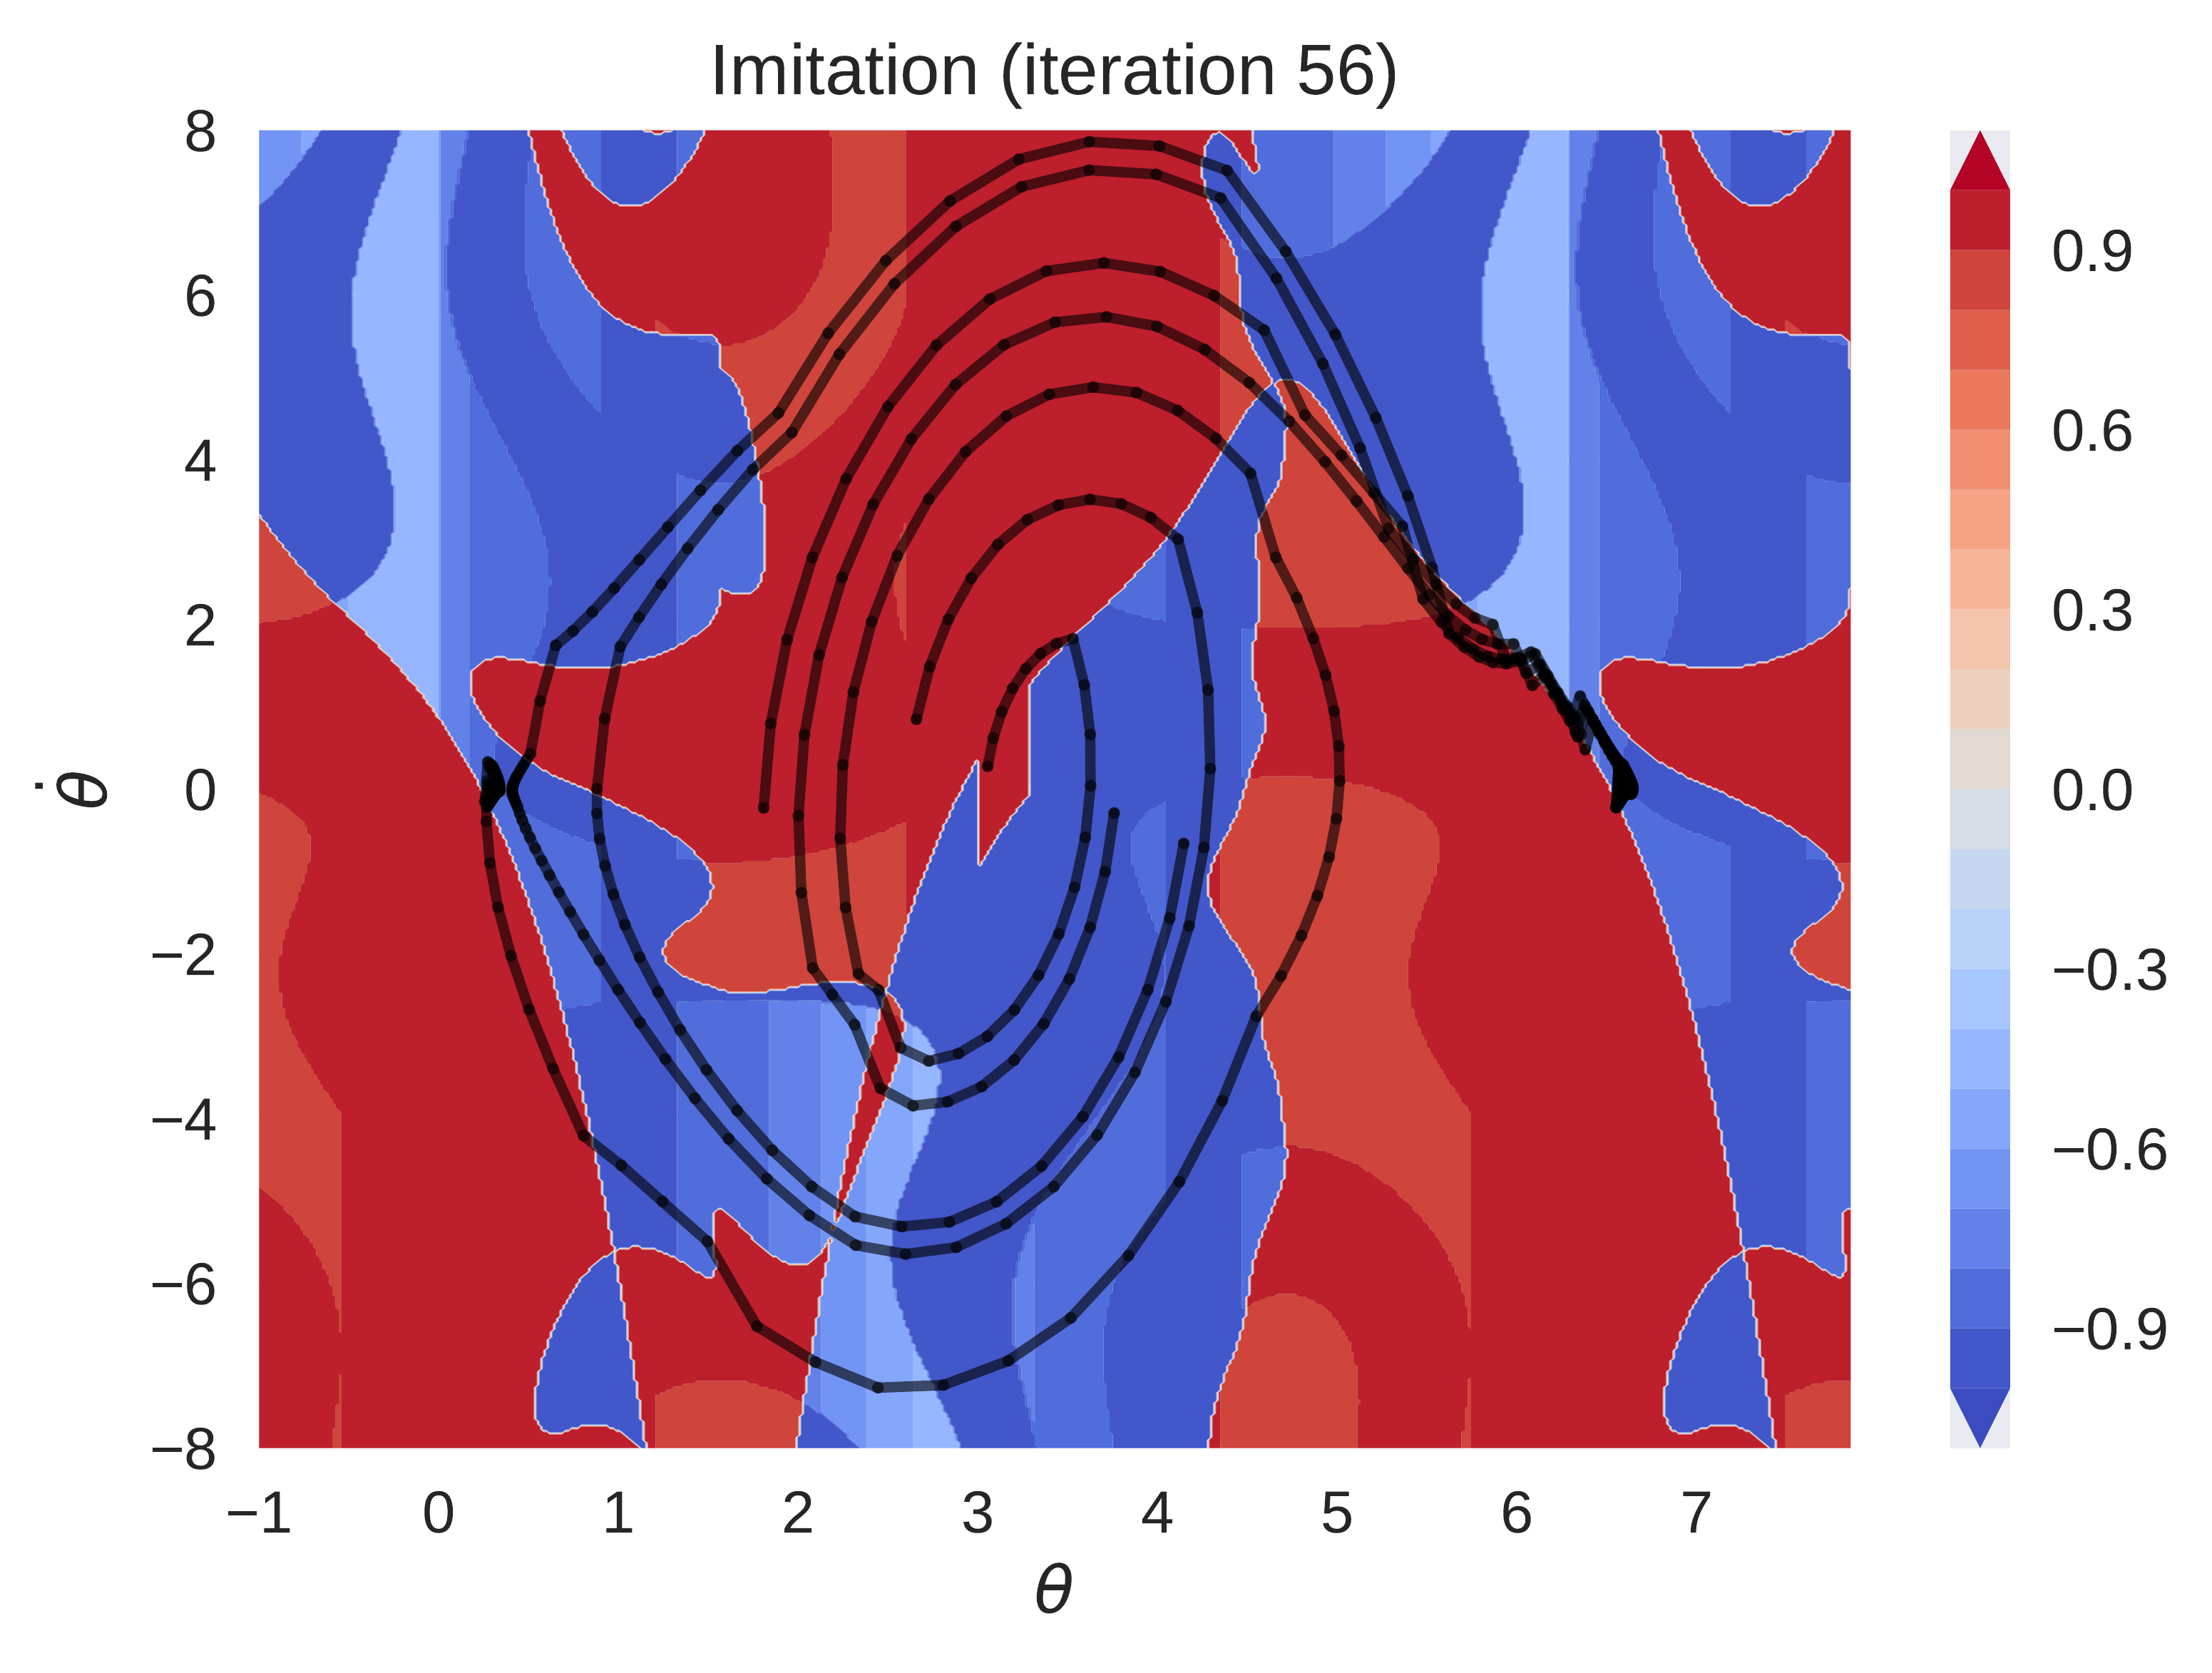
\includegraphics[width=0.37\textwidth]{images/imitation56.png}
    \end{figure}
    
\end{frame}

\begin{frame}{Summary}
    \begin{itemize}
        \item The Imitation-Projected Programmatic Reinforcement Learning framework integrates reinforcement learning with structured policy representations.
        \item We propose an extension to the framework, which we argue is key when scaling to more complicated structured spaces such as DSLs.
        \item Our experiments show that, despite using a simple local search heuristic which generates quite a few semantically identical candidates, interesting and/or complex solutions can be discovered across multiple iterations of interactive search.
    \end{itemize}
\end{frame}

\begin{frame}{Future work}
\begin{itemize}
    \item Integrate synthesis and learning steps, i.e. outer loop.
    \begin{itemize}
        \item How do we take advantage of discovered programs in the following reinforcement learning updates?
    \end{itemize}
    \item Examine policy decompositions and corresponding representations/DSLs.
    \begin{itemize}
        \item High-dimensional input processing.
        \item Decision making.
        \item Low-level control.
        \item Others?
    \end{itemize}
    \item Can certain reinforcement learning algorithms help discover structure better than others?
\end{itemize}
\end{frame}

\part{Causal state abstractions}
\frame[noframenumbering]{\centering\partpage\strut}
\section{Causal state abstractions}
\begin{frame}{Causal state abstractions}
    \begin{itemize}
        \item State abstraction or \enquote{coarse graining} is a key concept in RL.
        \item Any grouping or clustering of states is an \enquote{abstraction}.
        \item How to decide what is a good versus bad grouping?
        \bigskip
        \item \textbf{Key idea}: Causality is useful to measure abstraction quality.
    \end{itemize}

    \mybox{0.7, 0.5}{\fullcite{herlauReinforcementLearningCausal2022}}
\end{frame}

\begin{frame}{State abstractions}
\begin{itemize}
    \item Benefits include:
    \begin{itemize}
        \item More efficient computation and learning.
        \item Facilitate exploration and generalization.
        \item Synergy with composition and communication.
    \end{itemize}
\end{itemize}
    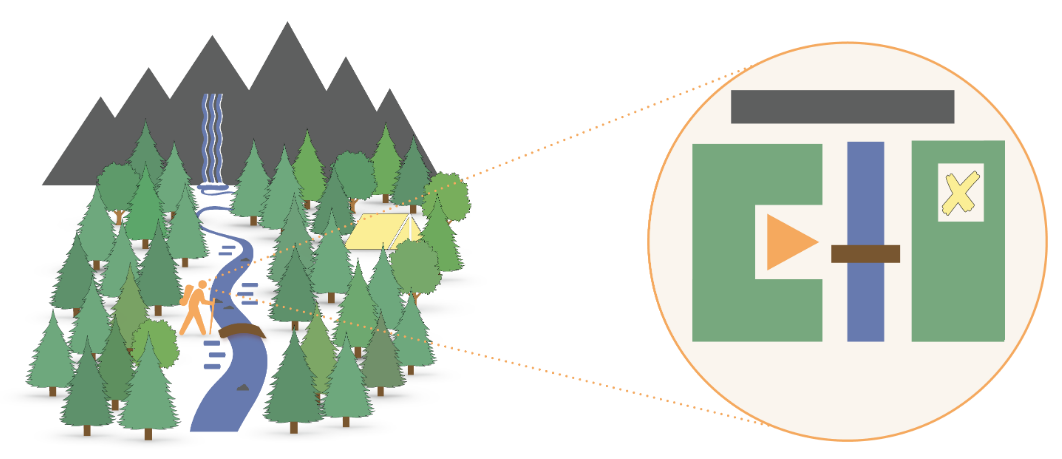
\includegraphics[width=0.58\textwidth]{images/valueofabstraction.png}
    \mybox{0.7, 0.45}{\fullcite{hoValueAbstraction2019}}
\end{frame}


\begin{frame}{Causality?}
    \begin{itemize}
        \item Fundamentally: \enquote{Nature} and the data it generates are intrinsically different.
        \item We model nature by having variables \enquote{listen} to their causes.
        \item Precisely formalized by Pearl and collaborators.
        \bigskip
        \item This implies a \textbf{causal hierarchy} or \textbf{ladder}.
    \end{itemize}
    
    %\begin{textblock}{0.4}(0.7, 0.5)\dbox{
    %\begin{minipage}{\dimexpr\textwidth-2\fboxsep-2\fboxrule\relax}
    %\scriptsize
    %\fullcite{pearlCausality2009a}
    %\end{minipage}}\end{textblock}
    \mybox{0.7, 0.5}{\fullcite{pearlCausality2009a}}
\end{frame}

\note[itemize]{
    \item But first off, what do I mean by causality?
}

\begin{frame}{Ladder of causation: seeing}
    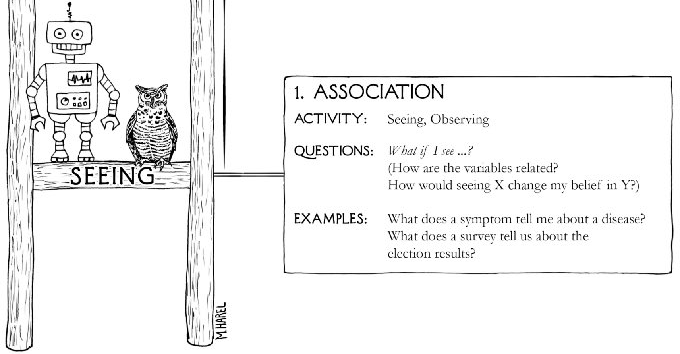
\includegraphics[width=0.9\textwidth]{images/ladder-of-causation-seeing.png}
    \mybox{0.7, 0.5}{\fullcite{pearlBookWhyNew2018}}
\end{frame}

\note{Layer 1 deals with purely “observational”, factual information}

\begin{frame}{Ladder of causation: doing}
    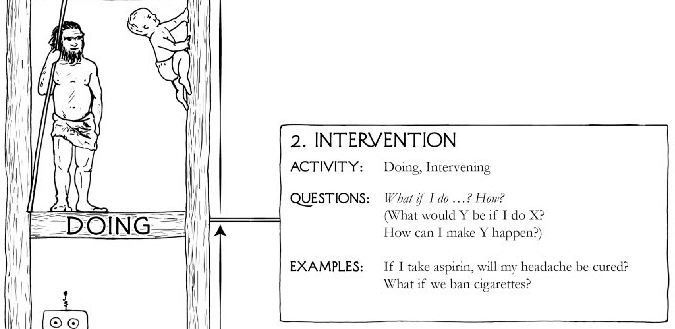
\includegraphics[width=0.9\textwidth]{images/ladder-of-causation-doing.png}
\end{frame}

\note[itemize]{
    \item Rung 2 encodes information about what would happen, hypothetically speaking, were some intervention to be performed, namely effects of actions.
}

\begin{frame}{Ladder of causation: imagining}
    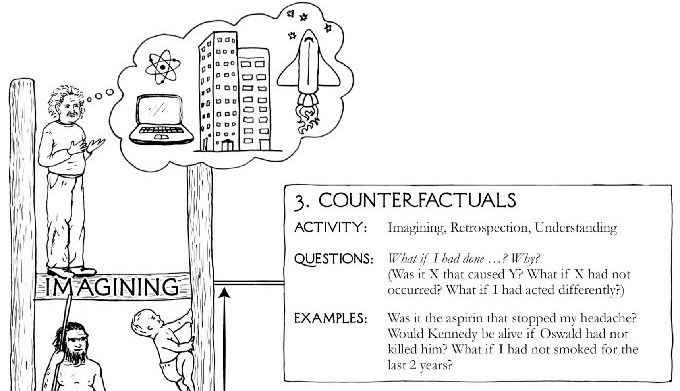
\includegraphics[width=0.88\textwidth]{images/ladder-of-causation-imagining.png}
\end{frame}

\note[itemize]{
    \item Finally, Layer 3 involves queries about what would have happened, counterfactually speaking, had some intervention been performed, given that something else in fact occurred (possibly conflicting with the hypothetical intervention). 
    \item The hierarchy establishes a useful classification of concepts that might be relevant for a given task, thereby also classifying formal frameworks in terms of the questions that they are able to represent, and ideally answer.
}

\begin{frame}{Some intuition on \enquote{causal} models}
    \begin{itemize}
        \item Not a binary concept: degrees of causality.
        \item Rung 2-causality: predictive accuracy of interventional queries.
        \item Rung 3-causality: predictive accuracy of counterfactual queries.
        \bigskip
        \item Humans have (sometimes) reasonably accurate counterfactual models!
    \end{itemize}
\end{frame}

\note[itemize]{
    \item So before moving on: my view
    \item I would not say a model is strictly "causal" or "not causal"
    \item Just like rung 1 associative models can be better or worse
    \item Models are still just models, some are more useful than others
    \item Intuition: Degrees of causality in models
    \item Corresponding to predictive accuracy
    \item Especially counterfactual accuracy can be hard to measure
    \item But humans manage to think and talk about counterfactuals every day
}

\begin{frame}{Structural Causal Models (SCMs)}
    \begin{itemize}
        \item An SCM consists of two sets of variables, $U$ and $V$, a distribution $P(U)$ and a set of mappings,
        \begin{equation*}
            v_i \leftarrow f_i(pa_i, u_i),
        \end{equation*}
        where $pa_i$ are the \emph{parents} of $v_i \in V$.
        \item The variables in $V$ are \emph{endogenous}, and are explicitly considered in the model, i.e. they are on the left hand side of one of the mappings.
        \item The variables in $U$ are \emph{exogenous}, and only appear in the functions $f_i$.
        \item For $Y \subseteq V$ in SCM $M$:
        \begin{equation*}
            P^M(y) = \sum_{\{u | Y(u) = y\}}P(u).
        \end{equation*}
        \item Every SCM is associated with a graph: nodes represent the variables in $U \cup V$, and directed edges represent the functions $f_i$.
    \end{itemize}
\end{frame}

\note[itemize]{
    \item Let's get into some formalities about causal models.
    \item SCMs are how we describe relevant aspects of the world.
    \item In essence, we assume that such an underlying data generating process exists, even though we cannot in general observe this process.
    \item The graph contains less information than the fully specified SCM: only which variables "listen" to others.
}


\begin{frame}{Queries in SCMs}
    \begin{itemize}
        \item For $X \subseteq V$, a \emph{submodel} $M_x$ of an SCM $M$ is
        \begin{equation*}
            M_x = \langle U, V, F_x, P(U) \rangle,
        \end{equation*}
        where
        \begin{equation*}
            F_x = \{f_i : V_i \notin X \} \cup \{X \leftarrow x\}.
        \end{equation*}
        \item The \emph{potential response} defines the rung 2 query,
        \begin{equation*}
            P(Y | do(X = x) = P^{M}(Y_x) = \sum_{\{u | Y_{M_x}(u) = y\}}P(u).
        \end{equation*}
        \item Rung 3 queries are defined, for counterfactual events $Y_x, \dots, Z_w$, as
        \begin{equation*}
            P^M(y_x, \dots, z_w) = \sum_{\{u | Y_{M_x}(u) = y, \dots, Z_{M_w}(u) = z\}}P(u).
        \end{equation*}
    \end{itemize}
\end{frame}

\note[itemize]{
    \item Just for the sake of it, let's quickly go through what it means to answer rung 2 and 3 queries.
    \item Rung 2: 
    \item Rung 3: note that the l.h.s. contain variables with different subscripts. These encode different counterfactual "worlds", and thus no experiment in the world (rung 2) is sufficient to answer the query. 
}

\begin{frame}{The causal agent}
    \includegraphics[width=.9\linewidth]{causal_figures/conceptA}
\end{frame}

\note[itemize]{
    \item This is our imagined setting - an agent possessing a causal model which is an abstraction over the states of the world.
    \item How would an agent go about acquiring a simple causal model of its environment?
    \item We're considering an RL setting, so of course the reward is important - we want to maximize it.
    \item Simultaneously, we want our choice in behavior to be considered with respect to how it affects the outcome.
    
}



\begin{frame}{Mediation analysis}
    \centering
    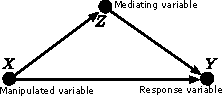
\includegraphics[width=0.4\linewidth]{causal_figures/medanal1}%\hspace{1cm}
    \begin{itemize}
        \item Mediation analysis deals with decompositions of effects into \emph{direct} and \emph{indirect} effects.
        \item The \emph{total} effect is $P(Y_x = y)$, as usually measured in randomized trials.
    \end{itemize}
    %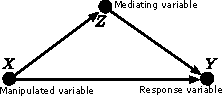
\includegraphics[width=0.4\linewidth]{causal_figures/medanal1}%\hspace{1cm}
    %\includegraphics[width=0.45\linewidth]{causal_figures/medanal2}
    %\begin{align*}
    %	\textrm{NIE} & = \left( \EE\left[Y | Z=1, \pi_a \right] - \EE\left[Y | Z=0, \pi_a \right] \right)  \\  
    %	& \times  \left( P(Z=1| \pi_b) -P(Z=1| \pi_a) \right).
    %\end{align*}
    \mybox{0.70, 0.47}{\fullcite{pearlDirectIndirectEffects2001}}
\end{frame}

\note[itemize]{
    \item ?
}

\begin{frame}{The natural indirect effect}
    \begin{itemize}
        \item An event $X = x$ is said to have an indirect effect on Y (in situation $U = u)$ if
        \begin{equation*}
            \mathrm{NIE}(u) = Y_{x', Z_x(u)}(u) \noteq Y_{x'}(u).
        \end{equation*}
        \item We can thus define the average indirect effect in general as
        \begin{equation*}
            \mathrm{NIE} = \E_u[Y_{x', Z_x(u)}(u)] - \E_u[Y_{x'}].
        \end{equation*}
        \item This is a \emph{nested} counterfactual and can only be identified in specific cases.
    \end{itemize}
\end{frame}

\note[itemize]{
    \item Now let's talk about the specific causal analysis that we use.
    \item The natural indirect effect, or just the indirect effect (since there is no controlled equivalent as in the direct effect), is:
    \item The value of Y changes when we keep X fixed at a reference $X = X'$ while changing Z to the value $Z_x$ that it would attain under $x$.
}

\begin{frame}{Identifying the NIE}
    \centering
    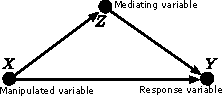
\includegraphics[width=0.5\linewidth]{causal_figures/medanal1}%\hspace{1cm}
    \begin{itemize}
        \item In this simple graph, the NIE is identified even without performing any experiments:
        \begin{equation*}
            \mathrm{NIE} = \sum_z\E[Y | x', z][P(z|x) - P(x | x')].
        \end{equation*}
    \end{itemize}
\end{frame}

\note[itemize]{
    \item This is under the condition that there exists a set $W$ of non-descendants of $X$ or $Z$ s.t. $Y_{x'z} \indep Z_x | W$.
}

\begin{frame}{Assigning variables}
    \centering
    \includegraphics[width=0.5\linewidth]{causal_figures/medanal2}
    
    \begin{itemize}
        \item With binary variables, the NIE further simplifies,
        \begin{align*}
        	\mathrm{NIE} & = \left( \E\left[Y | Z=1, \pi_a \right] - \E\left[Y | Z=0, \pi_a \right] \right)  \\  
        	& \times  \left( P(Z=1| \pi_b) -P(Z=1| \pi_a) \right).%\label{eq12}
        \end{align*}
    \end{itemize}

\end{frame}

\note[itemize]{
    \item Now we specify the meaning of variables in our simple mediation graph.
    \item Choosing binary variables further simplifies the NIE as well.
    \item In this form, we can easily understand what a high value of the NIE means:
    \item The first term relates to the reward outcome Y, and specifies that the causal state Z should be associated with a higher reward.
    \item The second term relates to the agents choice of policy, and specifies that the causal state should be more achievable with policy B. 
    \item As we'll see, policy A going to be a prespecified policy. 
}

\begin{frame}{Implementation: $Z$}
    \begin{itemize}
        \item We model $Z$ as a kind of \emph{stopped process}:
        \begin{equation*}
        	Z = \max\{Z_0, Z_1, \dots Z_T\}.
        \end{equation*}	
        \item Each $Z_t \in \{0,1\}$ is parameterized by a function approximator $\Phi$:
        \begin{equation*}
            Z_t \sim \textrm{Bern}(\Phi(s_t)).
        \end{equation*}
    \end{itemize}
\end{frame}

\note[itemize]{
    \item 
}

\begin{frame}{Implementation: $\pi$}
	\centering
	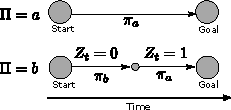
\includegraphics[width=0.4\linewidth]{causal_figures/medanal3}

	\begin{itemize}
    	\item The combined policy will either follow $\pi_a$, or follow the alternative policy $\pi_b$ until $Z$ is true after which it follows $\pi_a$. 
    \begin{align*}
    	\pi = \begin{cases} \pi_a & \mbox{if $\Pi = a$ } \\ \left(1-\max\{Z_{0}, \dots, Z_t\} \right)\pi_b +\max\{Z_{0}, \dots, Z_t\} \pi_a
    		& \mbox{if $\Pi = b$. }\end{cases} %\label{eq10}
    \end{align*}
	\end{itemize}	
\end{frame}

\note[itemize]{
    \item We implement the policy choice in a specific way.
    \item This is motivated by the term in the NIE that encourages $pi_b$ to reach $Z=1$.
    \item Additionally, the interpretation of $pi_b$ as part of a hierarchical policy is interesting.
}

\begin{frame}{Implementation: Maximization}
    \begin{itemize}
    	\item How to maximize the NIE wrt. $Z$ and $\pi_b$?
    	\begin{align*}
    		\mathrm{NIE} & = \left( \E\left[Y | Z=1, \pi_a \right] - \E\left[Y | Z=0, \pi_a \right] \right)  \\  
    		& \times  \left( P(Z=1| \pi_b) -P(Z=1| \pi_a) \right).%\label{eq12}
    	\end{align*}
    \item Estimate this quantity iteratively, in the same way as the Bellman iteration for the value function,
    \begin{equation*}
        V(s_{t} ) = \E[ R_{t+1} + \gamma V(s_{t+1}) | S_t=s_t].
    \end{equation*}

    \end{itemize}
\end{frame}

\note[itemize]{
    \item asd
}

\begin{frame}{Z-value functions}
We define the set of variables
\begin{equation*}
	Z_t^\infty = \max\{Z_t,Z_{t+1}, \dots,\}, %(1-Z_{k-1}) = \mbox{One of $Z_k,\dots$ is true and $Z_k$ is false}
\end{equation*}
each of which is $1$ at time $t$ if $Z$ becomes $1$ at any time $t$ or later -- and $0$ otherwise.
Our goal is then to estimate the quantities
\begin{align*}
	v^{\infty}_t(s_t) & = P(Z^\infty_t =1 | S_t=s_t, Z_{t-1} = 0), \\
	v^{z}_t(s_t) & = \E\left[G_t | S_t=s_t, Z_t^\infty = z, Z_{t-1} = 0\right],  %\label{eq19} 
\end{align*}
both of which are conditional on $Z_{t-1} = 0$.

These quantities satisfy mutually recursive equations which can be jointly estimated with standard algorithms.
%They satisfy recursions
%\begin{subequations} 
%\begin{align*}
%		v^\infty_t(s_t) & = \Phi(s_t) + (1-\Phi(s_t) ) \E\left[ v^\infty_{t+1}(S_{t+1} )| s_t\right],  \\ 
%		v^{1}_t(s_t) & =  \frac{ V(s_t) \Phi(s_t) }{V_t^\infty(s_t) }  
%		+ \frac{  1\!-\! \Phi(s_t)  }{V_t^\infty(s_t) } \E\left[ v^\infty_{t+1}(S_{t+1}) \left( R_{t+1} + \gamma v^{1}_{t+1}(S_{t+1} ) \right) \mid s_t   \right], \nonumber \\	
%\end{align*}
%\end{subequations}
%Both have the form
%\begin{align*}
%	v_t(s_t) & =\E\left[H_t(s_t,S_{t+1})  + G_t(s_t, S_{t+1}) v_{t+1}(S_{t+1} )  )  \middle| s_t\right] %\label{eq22a}
%\end{align*}
\end{frame}

\note[itemize]{
    \item The first denotes the event that $Z=1$ will happen in the future given that it has not yet.
    \item The second is the expected return given that Z has not happened yet, and that it will ($z=1$) or that it won't ($z=0$).
    \item Note that $v^\infty_0(s_0) = P(Z = 1| s_0)$ and $v^z_0(s_0) = \E[G_0 | s_0, Z=z]$.
    \item Luckily, those are also terms in our simplified NIE!
    \item 
}

\begin{frame}{Example: two-stage environment}
\centering
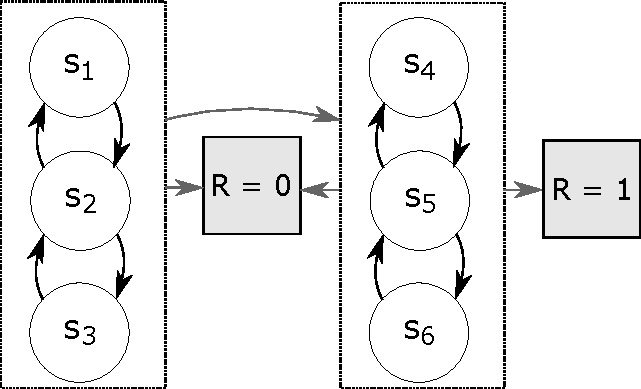
\includegraphics[width=.28\linewidth]{causal_figures/twostage}
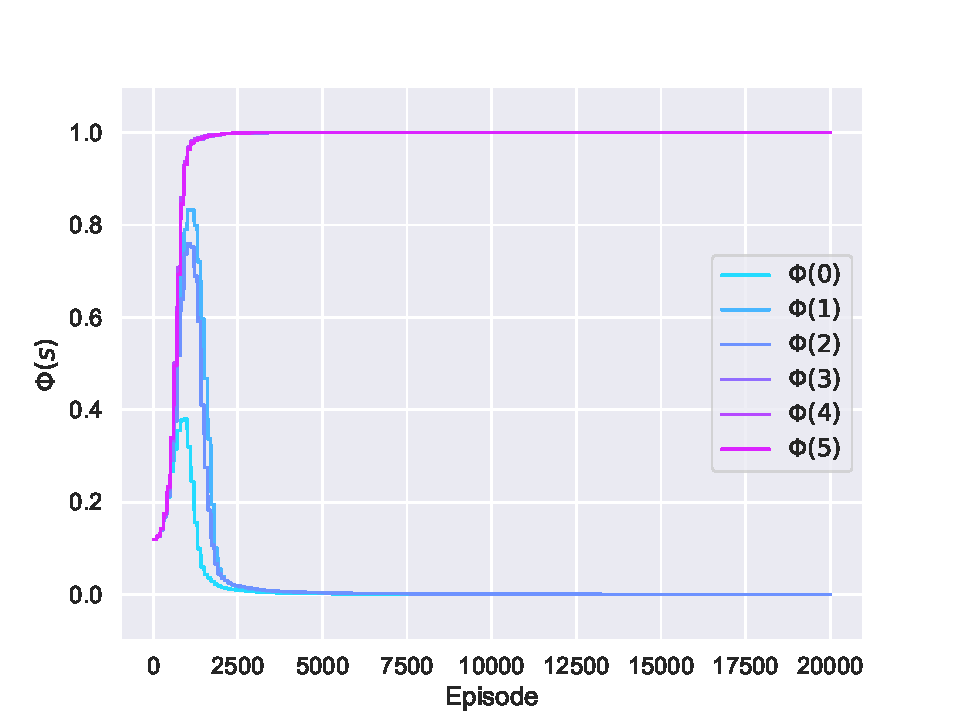
\includegraphics[width=.48\linewidth]{causal_figures/twostage_Phi}~
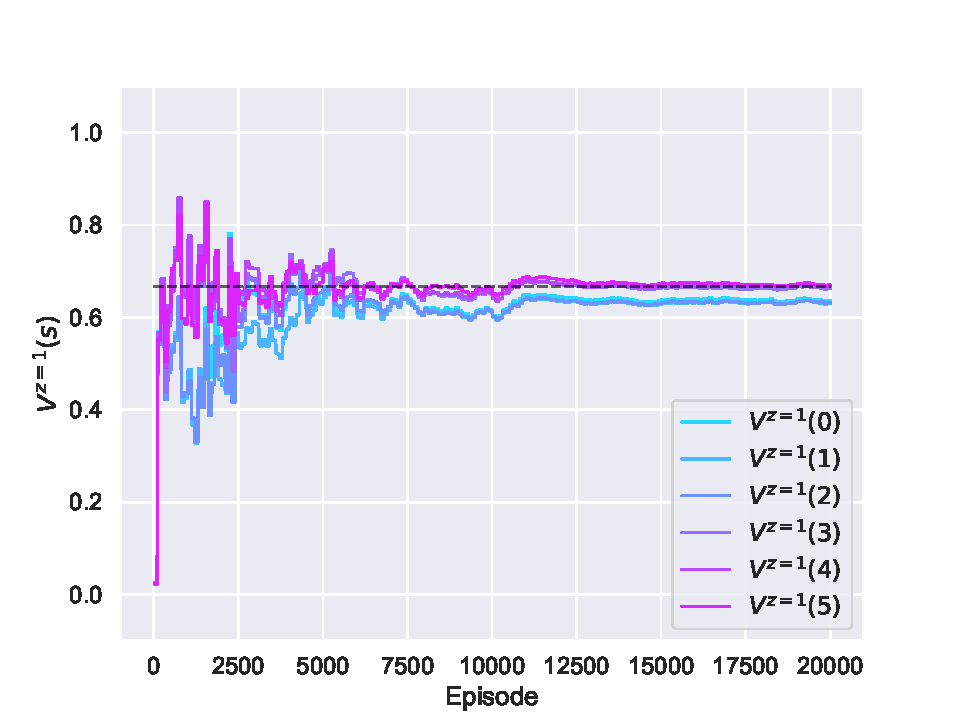
\includegraphics[width=.48\linewidth]{causal_figures/twostage_Vz1}
\end{frame}

\begin{frame}{Example: Doorkey environment}
\centering
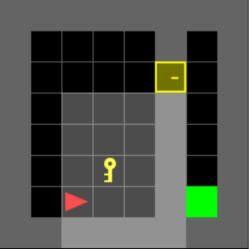
\includegraphics[width=.33\linewidth]{causal_figures/doorkey}~
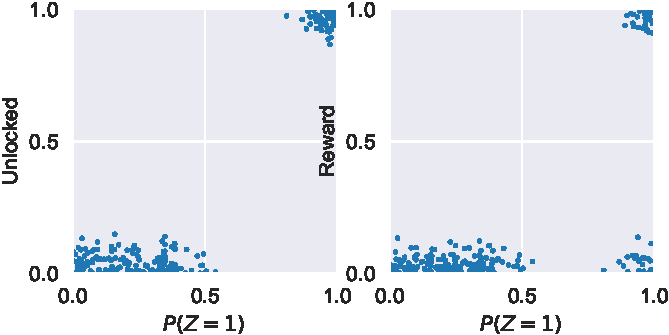
\includegraphics[width=0.66\linewidth]{causal_figures/scatter_AB}
\begin{itemize}
	\item Trained on a small Doorkey environment.
	\item Learned variable $Z$ corresponds to unlocking the door.
\end{itemize}
\end{frame}

\note[itemize]{
    \item Doorkey environment not shown, but pretty simple to explain.
    \item Left: Chance of unlocking door at each P(Z=1).
    \item Right: Chance of reaching goal state at each P(Z=1).
}

\begin{frame}\frametitle{Causality and optimal policies?}
    \begin{align*}
    	\mathrm{NIE} & = \left( \E\left[Y | Z=1, \pi_a \right] - \E\left[Y | Z=0, \pi_a \right] \right)  \\  
    	& \times  \left( P(Z=1| \pi_b) - P(Z=1| \pi_a) \right).%\label{eq12}
    \end{align*}
    \begin{itemize}
    \item The NIE will generally not be large when $\pi_a$ is optimal
    \item How well-defined is the notation of a parsimonious causal model when an optimal policy is known? 
    \end{itemize}
\end{frame}

\begin{frame}{Recent related work and future work}
    \begin{center}
        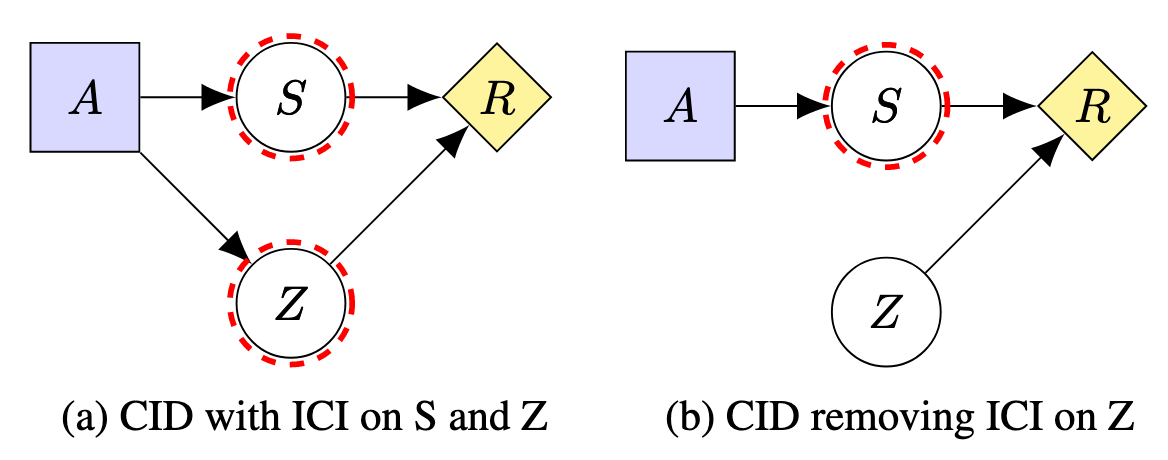
\includegraphics[width=.5\textwidth]{images/cid.png}
    \end{center}
    
    Future work:
    \begin{itemize}
    \item Unifying view of more concepts, e.g. agent safety using causality?
    \item Too heavy assumptions - can we remove some?
    \item Scaling up - sample efficiency and instability.
    \end{itemize}

    \mybox{0.01, 0.225}{\fullcite{farquharPathspecificObjectivesSafer2022}}
\end{frame}

\note[itemize]{
    \item I wanted to point out some related work that was also accepted at AAAI 2022.
    \item Here, Causal Influence Diagrams (as shown) describe a framework for safe training of agents whose \textbf{naive incentives} are unsafe.
    \item ICI = Instrumental Control Incentive, the red circles. Blue square is decision. Yellow diamond is utility. Black arrows show causal influence.
    \item Traditional RL obviously fails: expected return is maximized by any means.
    \item Their method trains agents by essentially optimizing only the \textbf{direct effect}, disallowing indirect effects through unsafe (aka delicate) causal states.
    \item Some future work for our setting:
    \item We use a simple setting in order for the NIE to be identifiable from *observational data* - but we aren't in a strictly observational setting. We can do experiments - which assumptions can we then remove, that we used to identify the NIE?
}






\section{Conclusion}
\begin{frame}{Conclusion}
\end{frame}

\end{document}